\section{Arquitetura Conceitual}

\subsection{Visão Geral}

A arquitetura conceitual proposta tem como objetivo introduzir uma camada de observabilidade e validação entre o Rest e o Integrador, sem alterar o comportamento principal da jornada do usuário final.

A solução deverá permitir que os fluxos atualmente executados pelo Rest possam ser comparados com os fluxos equivalentes implementados no Integrador, utilizando execução paralela, coleta de dados, comparação estruturada e visualização dos resultados em dashboard.

Em um primeiro momento, a arquitetura será direcionada ao suporte às migrações. Posteriormente, poderá evoluir para uma plataforma contínua de observabilidade das integrações com locadoras.

\subsection{Visão Conceitual do Fluxo}

O fluxo atual da transição de informações entre o Rest e o Integrador pode ser representado da seguinte forma:

\begin{figure}[H]
    \centering
    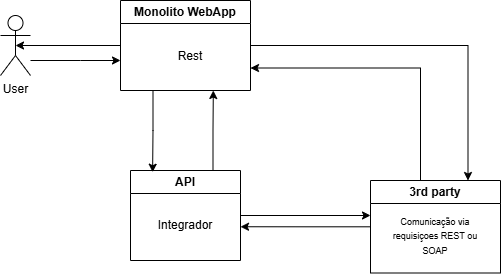
\includegraphics[width=0.6\textwidth]{assets/images/fluxo-atual.drawio.png}
    \caption{Fluxo atual de transição de informações entre Rest e Integrador}
    \label{fig:fluxo_atual}
\end{figure}

Durante o processo de validação, será adicionado um fluxo paralelo:

\begin{figure}[H]
    \centering
    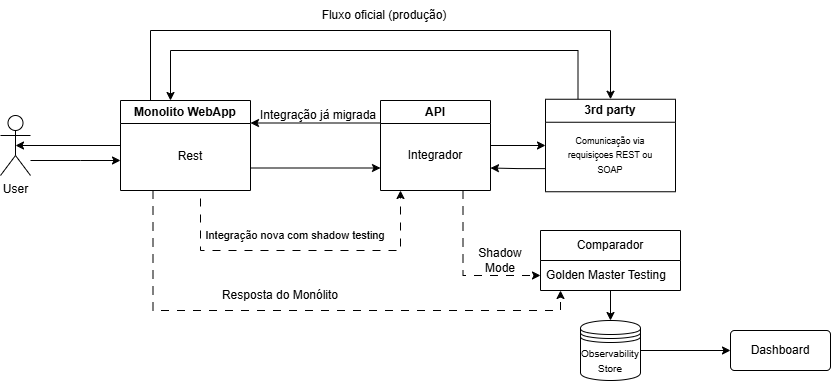
\includegraphics[width=0.8\textwidth]{assets/images/fluxo-proposto.drawio.png}
    \caption{Fluxo proposto de transição de informações entre Rest e Integrador}
    \label{fig:fluxo_proposto}
\end{figure}

Nesse modelo, o Rest continua sendo a fonte oficial da resposta ao usuário durante a fase de validação. O Integrador é executado em paralelo, sem interferir no resultado final apresentado ao cliente.

\subsection{Componentes Conceituais}

A arquitetura é composta pelos seguintes componentes principais:

\subsubsection{Rest}
Sistema responsável pelo fluxo atual das integrações ainda não migradas. Durante a fase de validação, atua como referência de comportamento para comparação com o Integrador.

\subsubsection{Integrador}
Gateway de integrações responsável por centralizar a comunicação com as locadoras. Representa o novo modelo arquitetural para implementação, evolução e manutenção das integrações.

\subsubsection{Shadow Mode Executor}
Componente responsável por permitir a execução paralela do fluxo no Integrador, sem impacto direto na resposta ao usuário final.

\subsubsection{Golden Master Comparator}
Componente responsável por comparar os resultados obtidos entre o fluxo legado e o fluxo executado pelo Integrador, identificando divergências funcionais relevantes.

\subsubsection{Camada de Persistência}
Responsável por armazenar os dados coletados durante as execuções, incluindo entradas, saídas, divergências, status da comparação e informações de rastreabilidade.

\subsubsection{Dashboard de Validação e Observabilidade}
Interface responsável por consolidar e apresentar os resultados das validações, permitindo acompanhar a evolução da migração por locadora, fluxo e criticidade das divergências encontradas.

\subsection{Modelo Conceitual de Dados}

De forma conceitual, o sistema deverá armazenar informações como:
\begin{itemize}
    \item Locadora
    \item Fluxo executado
    \item Identificador de correlação
    \item Dados de entrada (payloads enviados ao Rest e ao Integrador)
    \item Dados de saída (respostas recebidas do Rest e do Integrador)
    \item Resultado da comparação (concordância ou divergência)
    \item Detalhes das divergências encontradas
    \item Timestamp das execuções
    \item Status geral da validação por fluxo e locadora
\end{itemize}

Esses dados permitirão rastrear o comportamento das integrações, identificar padrões de falha e apoiar decisões sobre a prontidão de cada locadora para migração.

\subsection{Papel da Arquitetura no Processo de Migração}

A arquitetura proposta atua como um mecanismo de redução de risco durante a migração dos drivers e locadoras. Ao permitir a comparação entre o comportamento legado e o novo comportamento no Integrador, o sistema cria uma base objetiva para responder perguntas como:
\begin{itemize}
    \item O driver/locadora está pronto para migrar?
    \item Quais fluxos ainda apresentam divergências?
    \item  As divergências são críticas ou aceitáveis?
    \item O Integrador está reproduzindo corretamente o comportamento esperado?
    \item Há impacto potencial em reservas, disponibilidade ou receita?
\end{itemize}

Dessa forma, a arquitetura não apenas apoia a execução técnica da migração, mas também melhora a governança, a previsibilidade e a confiabilidade do processo.

